\iffalse
This file is protected by Copyright. Please refer to the COPYRIGHT file
distributed with this source distribution.

This file is part of OpenCPI <http://www.opencpi.org>

OpenCPI is free software: you can redistribute it and/or modify it under the
terms of the GNU Lesser General Public License as published by the Free Software
Foundation, either version 3 of the License, or (at your option) any later
version.

OpenCPI is distributed in the hope that it will be useful, but WITHOUT ANY
WARRANTY; without even the implied warranty of MERCHANTABILITY or FITNESS FOR A
PARTICULAR PURPOSE. See the GNU Lesser General Public License for more details.

You should have received a copy of the GNU Lesser General Public License along
with this program. If not, see <http://www.gnu.org/licenses/>.
\fi

% AV-5479: Assume this is in projects/assets_ts of source checkout
\def\importpath{../../../../assets/components/dsp_comps/fir_complex_sse.test/doc/}
\makeatletter
\def\input@path{{\importpath/snippets/}}
\makeatother
\documentclass{article}
\iffalse
This file is protected by Copyright. Please refer to the COPYRIGHT file
distributed with this source distribution.

This file is part of OpenCPI <http://www.opencpi.org>

OpenCPI is free software: you can redistribute it and/or modify it under the
terms of the GNU Lesser General Public License as published by the Free Software
Foundation, either version 3 of the License, or (at your option) any later
version.

OpenCPI is distributed in the hope that it will be useful, but WITHOUT ANY
WARRANTY; without even the implied warranty of MERCHANTABILITY or FITNESS FOR A
PARTICULAR PURPOSE. See the GNU Lesser General Public License for more details.

You should have received a copy of the GNU Lesser General Public License along
with this program. If not, see <http://www.gnu.org/licenses/>.
\fi

\author{} % Force author to be blank
%----------------------------------------------------------------------------------------
% Paper size, orientation and margins
%----------------------------------------------------------------------------------------
\usepackage{geometry}
\geometry{
	letterpaper,			% paper type
	portrait,				% text direction
	left=.75in,				% left margin
	top=.75in,				% top margin
	right=.75in,			% right margin
	bottom=.75in			% bottom margin
 }
%----------------------------------------------------------------------------------------
% Header/Footer
%----------------------------------------------------------------------------------------
\usepackage{fancyhdr} \pagestyle{fancy} % required for fancy headers
\renewcommand{\headrulewidth}{0.5pt}
\renewcommand{\footrulewidth}{0.5pt}
\rhead{\small{ANGRYVIPER Team}}
%----------------------------------------------------------------------------------------
% Appendix packages
%----------------------------------------------------------------------------------------
\usepackage[toc,page]{appendix}
%----------------------------------------------------------------------------------------
% Defined Commands & Renamed Commands
%----------------------------------------------------------------------------------------
\renewcommand{\contentsname}{Table of Contents}
\renewcommand{\listfigurename}{List of Figures}
\renewcommand{\listtablename}{List of Tables}
\newcommand{\todo}[1]{\textcolor{red}{TODO: #1}\PackageWarning{TODO:}{#1}} % To do notes
\newcommand{\code}[1]{\texttt{#1}} % For inline code snippet or command line
%----------------------------------------------------------------------------------------
% Various pacakges
%----------------------------------------------------------------------------------------
\usepackage{hyperref} % for linking urls and lists
\usepackage{graphicx} % for including pictures by file
\usepackage{listings} % for coding language styles
\usepackage{rotating} % for sideways table
\usepackage{pifont}   % for sideways table
\usepackage{pdflscape} % for landscape view
%----------------------------------------------------------------------------------------
% Table packages
%----------------------------------------------------------------------------------------
\usepackage{longtable} % for long possibly multi-page tables
\usepackage{tabularx} % c=center,l=left,r=right,X=fill
\usepackage{float}
\floatstyle{plaintop}
\usepackage[tableposition=top]{caption}
\newcolumntype{P}[1]{>{\centering\arraybackslash}p{#1}}
\newcolumntype{M}[1]{>{\centering\arraybackslash}m{#1}}
%----------------------------------------------------------------------------------------
% Block Diagram / FSM Drawings
%----------------------------------------------------------------------------------------
\usepackage{tikz}
\usetikzlibrary{shapes,arrows,fit,positioning}
\usetikzlibrary{automata} % used for the fsm
%----------------------------------------------------------------------------------------
% Colors Used
%----------------------------------------------------------------------------------------
\usepackage{colortbl}
\definecolor{blue}{rgb}{.7,.8,.9}
\definecolor{ceruleanblue}{rgb}{0.16, 0.32, 0.75}
\definecolor{drkgreen}{rgb}{0,0.6,0}
\definecolor{deepmagenta}{rgb}{0.8, 0.0, 0.8}
\definecolor{cyan}{rgb}{0.0,0.6,0.6}
\definecolor{maroon}{rgb}{0.5,0,0}

%----------------------------------------------------------------------------------------
% Update the docTitle and docVersion per document
%----------------------------------------------------------------------------------------
\def\docTitle{Component Data Sheet}
\def\docVersion{1.5}
%----------------------------------------------------------------------------------------
\date{Version \docVersion} % Force date to be blank and override date with version
\title{\docTitle}
\lhead{\small{\docTitle}}

\def\comp{fir\_complex\_sse\_ts}
\edef\ecomp{fir_complex_sse_ts}
\def\Comp{FIR Complex SSE (TimeStamped)}
\graphicspath{ {\importpath/figures/} }

\begin{document}

\section*{Summary - \Comp}

\begin{tabular}{|c|M{13.5cm}|}
	\hline
	\rowcolor{blue}
	                  &                                                              \\
	\hline
	Name              & \comp                                                        \\
	\hline
	Worker Type       & Application                                                  \\
	\hline
	Version           & v\docVersion \\
	\hline
	Release Date      & 4/2019 \\
	\hline
	Component Library & ocpi.assets\_ts.components                                        \\
	\hline
	Workers           & \comp.hdl                                                    \\
	\hline
	Tested Platforms  & xsim, isim, modelsim, Matchstiq-Z1(PL) \\
	\hline
\end{tabular}

\section*{Functionality}
\begin{flushleft}
	The FIR Complex SSE (Systolic Symmetric Even) component inputs complex signed samples and filters them based upon a programmable number of coefficient tap values. The worker also processes all operations of the Complex\_Short\_With\_Metadata protocol, passing along time and interval information. The underlying FIR Filter implementation makes use of a symmetric systolic structure to construct a filter with an even number of taps and symmetry about its midpoint.
\end{flushleft}

\section*{Worker Implementation Details}
\subsection*{\comp.hdl}
\begin{flushleft}
	The \verb+NUM_TAPS_p+ parameter defines the number of coefficient values. Care should be taken to ensure that the \verb+COEFF_WIDTH_p+ parameter is $\le$ the type (size) of the taps property. The taps property is type short, so \verb+COEFF_WIDTH_p+ must be between 1 and 16. Identical filter tap coefficients are applied to both real and imaginary input samples.\medskip

	This implementation uses \verb+NUM_TAPS_p/2+ multipliers for each of the real and imaginary data paths and processes input data at the clock rate - i.e. this worker can handle a new input value every clock cycle.\medskip

	The FIR Complex SSE worker utilizes the OCPI \textit{Complex\_Short\_With\_Metadata} protocol for both input and output ports. The \textit{Complex\_Short\_With\_Metadata} protocol conveys sample data using an interface of 16-bit complex signed samples. The \verb+DATA_WIDTH_p+ parameter may be used to restrict the the number of bits processed on the input and the number of bits (sign-extended) produced on the input.
\end{flushleft}
{\centering\captionsetup{type=figure}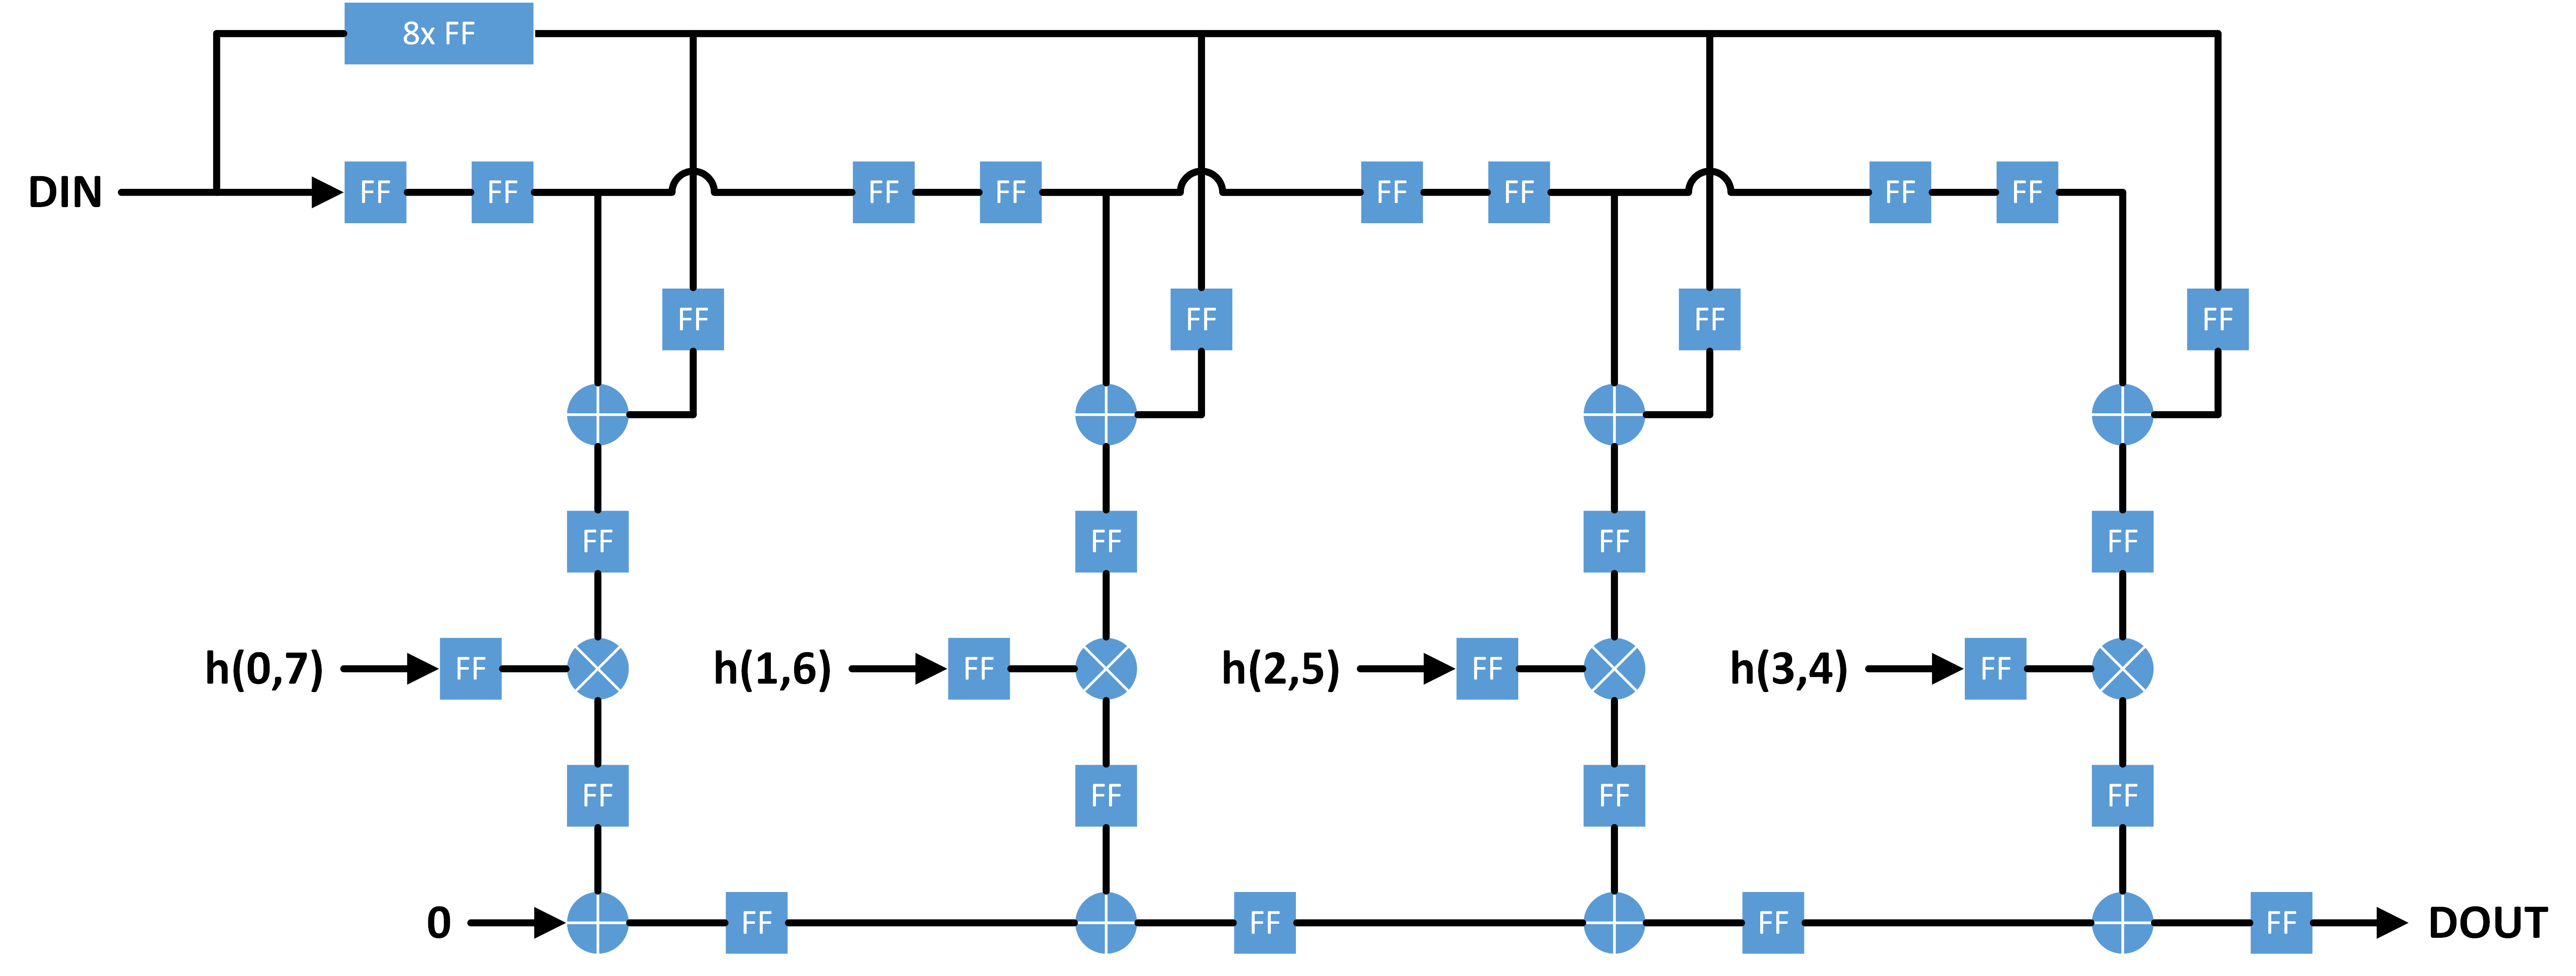
\includegraphics[scale=0.65]{fir_systolic_sym_even}\par\captionof{figure}{FIR Complex SSE Block Diagram - 8-tap example per I/Q rail}\label{fig:circuit}}

\section*{Theory}
\begin{flushleft}
	For a FIR filter with symmetric impulse response we are guaranteed to have linear phase response and thus constant group delay vs. frequency. In general, the group delay will be equal to (\verb+NUM_TAPS_p+-1)/2.	The filter topology itself will add some propagation delay to the response. For this design the total delay from an impulse input to the beginning of the impulse response will be \verb+NUM_TAPS_p/2+ + 4 samples.\medskip

	The worker only outputs samples after the delay has occurred. During \verb+flush+ or \verb+done+ operations, the worker continues to produce valid data until the pipeline is empty. During the \verb+sync+ operation, the pipeline is emptied, but no valid data is produced. During \verb+flush+, \verb+done+, and \verb+sync+ operations, the operation is passed along after the pipeline is empty.\medskip

	The worker passes along and does not modify \verb+time+ and \verb+interval+ operations.
\end{flushleft}

\section*{Block Diagrams}
\subsection*{Top level}
\begin{center}
	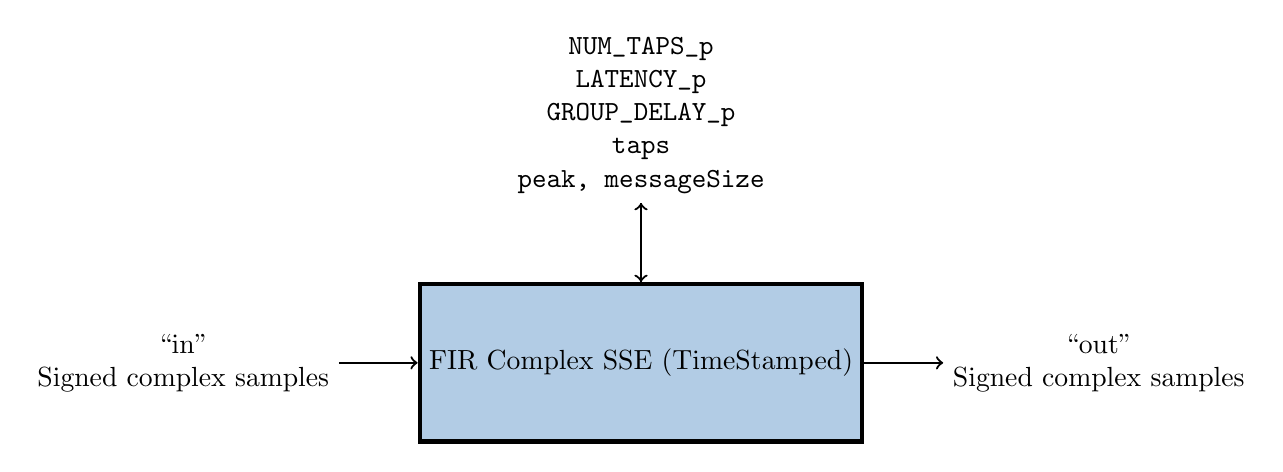
\begin{tikzpicture}[% List of styles applied to all, to override specify on a case-by-case
			every node/.style={
				align=center,  		% use this so that the "\\" for line break works
				minimum size=2cm	% creates space above and below text in rectangle
			},
			every edge/.style={draw,thick}
		]
		\node[rectangle,ultra thick,draw=black,fill=blue](R2){\Comp};
		\node[rectangle,draw=white,fill=white](R3)[left= of R2]{``in'' \\ Signed complex samples};
		\node[rectangle,draw=white,fill=white](R4)[right= of R2]{``out'' \\ Signed complex samples};
		\node[rectangle,draw=white,fill=white](R5)[above= of R2]{\verb+NUM_TAPS_p+ \\ \verb+LATENCY_p+ \\ \verb+GROUP_DELAY_p+ \\ \verb+taps+ \\ \verb+peak, messageSize+};
		\path[->]
		(R3)edge []	node [] {} (R2)
		(R2)edge []	node [] {} (R4)
		(R2)edge []	node [] {} (R5)
		(R5)edge []	node [] {} (R2)
		;
	\end{tikzpicture}
\end{center}

\section*{Source Dependencies}
\subsection*{\comp.hdl}
\begin{itemize}
	\item projects/assets\_ts/components/fir\_complex\_sse.hdl/fir\_complex\_sse.vhd
          	\item projects/assets/hdl/primitives/dsp\_prims/dsp\_prims\_pkg.vhd
	      \subitem projects/assets/hdl/primitives/dsp\_prims/fir/src/fir\_systolic\_sym\_even.vhd
	      \subitem projects/assets/hdl/primitives/dsp\_prims/fir/src/macc\_systolic\_sym.vhd
	\item projects/assets/hdl/primitives/misc\_prims/misc\_prims\_pkg.vhd
	      \subitem projects/assets/hdl/primitives/misc\_prims/round\_conv/src/round\_conv.vhd
	\item projects/assets/hdl/primitives/util\_prims/util\_prims\_pkg.vhd
	      \subitem projects/assets/hdl/primitives/util\_prims/pd/src/peakDetect.vhd

\end{itemize}

\begin{landscape}
	\section*{Component Spec Properties}
	\begin{scriptsize}
		\begin{tabular}{|p{1.5cm}|p{1cm}|c|c|c|p{3cm}|c|p{7cm}|}
			\hline
			\rowcolor{blue}
			Name               & Type   & SequenceLength & ArrayDimensions   & Accessibility	& Valid Range                                                                      & Default & Usage                                                                        \\
			\hline
			\verb+NUM_TAPS_p+  & ULong  & -              & -                 & Parameter		& 1-?                                                                              & 16      & Number of coefficients used by each real/imag even symmetric filter \\
			\hline
			\verb+peak+        & Short  & -              & -                 & Volatile		& Standard                                                                         & 0       & Read-only amplitude which may be useful for gain control                     \\
			\hline
			\verb+taps+        & Short  & -              & \verb+NUM_TAPS_p+ & Writable		& -2\textsuperscript{COEFF\_WIDTH\_p-1} to +2\textsuperscript{COEFF\_WIDTH\_p-1}-1 & -       & Symmetric filter coefficient values loaded into both real/imag filters       \\
			\hline
		\end{tabular}
	\end{scriptsize}

	\section*{Worker Properties}
	\subsection*{\comp.hdl}
	\begin{scriptsize}
		\begin{tabular}{|p{3cm}|p{2cm}|p{1cm}|c|c|c|c|c|p{5cm}|}
			\hline
			\rowcolor{blue}
			Type     & Name                 & Type  	& SequenceLength & ArrayDimensions & Accessibility	& Valid Range & Default & Usage                                        \\
			\hline
			Property & \verb+DATA_WIDTH_p+  & -     	& -              & -               & Parameter		& 1-16        & 16      & Number of bits of input data which are processed by FIR primitive \\
			\hline
			Property & \verb+COEFF_WIDTH_p+ & -	 	& -              & -               & Parameter		& 1-32        & 16      & Number of bits of taps property values which are processed by FIR primitive\\
			\hline
			Property & \verb+LATENCY_p+ 	 & UShort	& -              & -               & Parameter		& -           & 1       & Clock cycle delay between input and output   \\
			\hline
			Property & \verb+GROUP_DELAY_p+ & -		& -              & -               & Parameter		& -           & 1       & Number of clocks between first valid input and first valid output\\
			\hline
		\end{tabular}
	\end{scriptsize}


	\section*{Component Ports}
	\begin{scriptsize}
		\begin{tabular}{|M{2cm}|M{1.5cm}|M{4cm}|c|c|M{9cm}|}
			\hline
			\rowcolor{blue}
			Name & Producer & Protocol           					& Optional & Advanced & Usage                  \\
			\hline
			in   & false    & Complex\_Short\_With\_Metadata		& false    & -        & Complex signed samples \\
			\hline
			out  & true     & Complex\_Short\_With\_Metadata		& false    & -        & Complex signed samples \\
			\hline
		\end{tabular}
	\end{scriptsize}

	\section*{Worker Interfaces}
	\subsection*{\comp.hdl}
	\begin{scriptsize}
		\begin{tabular}{|M{2cm}|M{1.5cm}|c|c|M{12cm}|}
			\hline
			\rowcolor{blue}
			Type            & Name & DataWidth & Advanced  & Usage                  \\
			\hline
			StreamInterface & in   & 32        & 			& Signed complex samples \\
			\hline
			StreamInterface & out  & 32        & 			& Signed complex samples \\
			\hline
		\end{tabular}
	\end{scriptsize}
\end{landscape}

\section*{Control Timing and Signals}
\begin{flushleft}
	The FIR Complex SSE worker uses the clock from the Control Plane and standard Control Plane signals. The Raw Property interface is used to read/write coefficient values.
\end{flushleft}

\begin{landscape}
\section*{Worker Configuration Parameters}
\subsubsection*{\comp.hdl}
\input{../../\ecomp.hdl/configurations.inc}
\section*{Performance and Resource Utilization}
\subsubsection*{\comp.hdl}
\input{../../\ecomp.hdl/utilization.inc}
\end{landscape}

\section*{Test and Verification}

\begin{flushleft}
A single test case is implemented to validate the FIR Complex SSE component. The python script \textit{gen\_lpf\_taps.py} is used to generate a taps file consisting of \verb+NUM_TAPS_p/2+ filter coefficients. Input data is generated by first creating a *.dat input file containing all of the opcodes of the Complex\_Short\_With\_Metadata protocol in the following sequence:
\begin{enumerate}
	\item Interval
	\item Sync (this opcode is expected after an Interval opcode)
	\item Time
	\item Samples (impulse with length numtaps*2)
	\item Samples (impulse with length numtaps*2)
	\item Flush
	\item Samples (impulse with length numtaps*2)
	\item Sync
	\item Samples (impulse with length numtaps*2)
\end{enumerate}

The samples messages consist of a single maximum signed value of +32767 (for each real/imag filter) followed by 2*(\verb+NUM_TAPS_p+-1) zero samples (again for each real/imag filter). The *.bin input file is the binary version of the *.dat ASCII file repeated \verb+NUM_TAPS_p+ times.\medskip

The FIR Complex SSE worker inputs complex signed samples, filters the input as defined by the coefficient filter taps, and outputs complex signed samples. Since the input consists of an impulse response - that is, a maximal `one' sample followed by all zeros equal to the length of the filter - the output of each filter is simply the coefficient values.\medskip

The worker will pass through the interval and time opcodes. The samples opcode followed by flush or done will output an impulse response, showing the symmetric tap values. The samples opcode followed by sync will produce the first numtaps*2-group\_delay tap values. In addition to the samples data, the worker also passes along the zlms.\medskip

For verification, the output file is parsed into messages. All non-samples messages should match the input exactly. The samples messages are compared to the tap values and checked to ensure they are within +/- 1.
\end{flushleft}
\end{document}
